\section{The Kalman Filter}

While object detection algorithms operate at rates of less than 10 Hz when run on the Movidius NCS, the controller for a rotating camera necessitates a higher frequency. In addition, it would be useful to be able to estimate a likely position for the object in cases where the object detection algorithm fails.

The Kalman Filter (and its nonlinear variant, the Extended Kalman Filter), can solve both of these problems \cite{kalman1960new}.

\subsection{An brief introduction to the Kalman Filter}
A Kalman Filter is an algorithm used to estimate the state of a linear system ($\hat{x}$) along with the uncertainty of the estimate ($P$) based on measurements over time ($z$). The measurements are assumed to include noise with covariance $R$. It makes use of a model of the system ($F$) which represents the dynamics of the system ($\hat{x}_{k} = F\hat{x}_{k-1}$), along with a model which represents inaccuracies in the model, dubbed 'process noise' ($Q$) and measured factors which affect the state, but aren't part of the current set of states ($u$). It takes into account the sensor scaling which maps from between sensor measurements and state values ($H$). The notation for Kalman Filters has not been totally standardised.

A variety of excellent resources exist which explain the deeper intuition behind the Kalman Filter \cite{website:wlu_kalman_tutorial, website:bzarg_kalman_tutorial}. Thus, only the equations and high-level concepts which are absolutely necessary will be discussed in this chapter.

Kalman Filters continuously alternate between a predict stage and an update stage. In the predict stage, the Kalman Filter uses a model of the system and known disturbances to update the state estimate and uncertainty estimate. These are represented by the equations,

\[ \hat{x}_k = F_k \hat{x}_{k-1} + B_k u_k \]
\[ P_k = F_k P_{k-1} F_k^T + Q_k \]

The $k$ subscripts denote the point in time at which the calculation takes place. This means that any matrix in the algorithm could be updated as time goes on.

In the 'update' stage, the Kalman Filter makes use of a model of uncertainty estimates to produce a new state estimate which is a trade-off between new data from a sensor, and the state estimate produced by the predict stage.

\[ \hat{x}_k = \hat{x}_{k-1} + K_k (z_k - H_k x_{k-1}) \]
\[ P_k = (I - K_k H_k) P_{k-1} \]

where the Kalman gain $K$ at a time $k$ is calculated as,
\[ K_k = P_k H_k^T (H_k P_k H_k^T + R_k)^{-1} \]

%These stages are alternated as \emph{predict} $\rightarrow$ \emph{update} $\rightarrow$ \emph{predict} $\rightarrow$ \dots
As an illustration, consider the extremes during the update stage: when $K = 0$, we have

\[ \hat{x}_k = \hat{x}_{k-1} + 0 (z_k - H_k x_k) = \hat{x}_{k-1} \]

If $H_k = 1$ and $K = 1$, we have

\[ \hat{x}_k = \hat{x}_{k-1} + (z_k - x_k) = z_k \]

Values of $K$ in between result in a state update which is some combination of the sensed values and modelled dynamics of the system. Thus, the role of the Kalman Filter is essentially to find the optimal trade off between trusting the model and trusting the sensor readings. An illustration of this is shown below, in Figure~\ref{fig:kalman_filter_loop}.

\begin{figure}[h!]
  \centering
  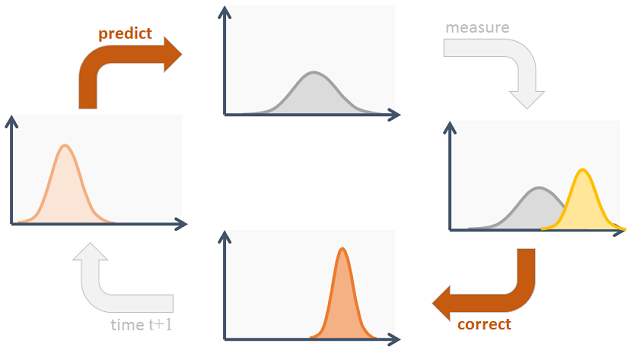
\includegraphics[width=0.6\textwidth]{literature_review/kalman_filter_loop}
  \caption{\label{fig:kalman_filter_loop}An illustration showing how the mean and covariance of an estimate (as predicted by the Kalman Filter) changes during the predict and update stages \cite{website:kalman_visualisation}.}
\end{figure}


Finally, given a Kalman Filter with an accurate estimation of systems state and a model which adequately predicts the future state of the system, one can interpolate between readings from a sensor with slow update rates. This could mean getting model updates at a required speed of 20 Hz using a sensor which only makes measurements at a rate of 5 Hz.


\subsection{An introduction to the Extended Kalman Filter}
An Extended Kalman Filter (EKF) is simply a nonlinear version of a Kalman Filter, where the transition from estimated state $\hat{x}_{k-1}$ to state $\hat{x}_k$ is some \emph{nonlinear} mapping $f(x)$ and the mapping from state values to sensor values is a nonlinear function $h(x)$. It works by using a Taylor approximation to linearize about an estimate of the current mean and covariance. This also results in differing values for their respective Jacobian matrices.

\[ F \hat{x} \rightarrow f(\hat{x}) \qquad H \hat{x} \rightarrow h(\hat{x}) \]

To understand the effects of this, consider the following: given a sensor which maps from state to measurement following the function $h(x) = x^2 - 10\cos{(x)}$, reading a value of $x = 8.5$ when the state was actually $x=7.5$ would result in an absolute error of $25.5$. However, reading a value of $x=4.5$ when the state was actually $x=3.5$ would result in an absolute error of $0.743$. Clearly, the same one unit error (due to noise, for example) should be treated differently depending on where it happens on the sensor curve. The EKF does just this! Code to create the plot can be found on the authors \href{https://github.com/alknemeyer/EEE4022S-Thesis-Project/blob/master/Final%20code/Illustrations%20for%20report.ipynb}{GitHub repository}.

\begin{figure}[h!]
  \centering
  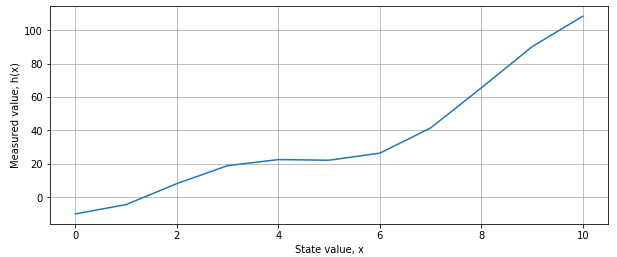
\includegraphics[width=0.7\textwidth]{literature_review/EKF_nonlinear_sensor}
  \caption{\label{fig:EKF_nonlinear_sensor}A plot of a hypothetical nonlinear sensor which maps state to measured value according to the function $h(x) = x^2 - 10\cos{(x)}$.}
\end{figure}

Thus, an EKF would update its covariance estimates in a different way depending on the part of the sensor/prediction curve it finds itself on.

Implementation-wise, the only difference between the linear and non-linear variants of the Kalman Filter is that the state transition and observation models can be non-linear differentiable functions with constantly updating Jacobians.

